
\section{Instalar y Configurar CENTOS 6.2 DESKTOP}

\begin{itemize}
\item PASO 15:
\\Una vez cargada esta ventana seleccionamos la primera opción para realizar la instalación de CentOS 6.2  con las teclas direccionales y enter.
		\begin{center}
		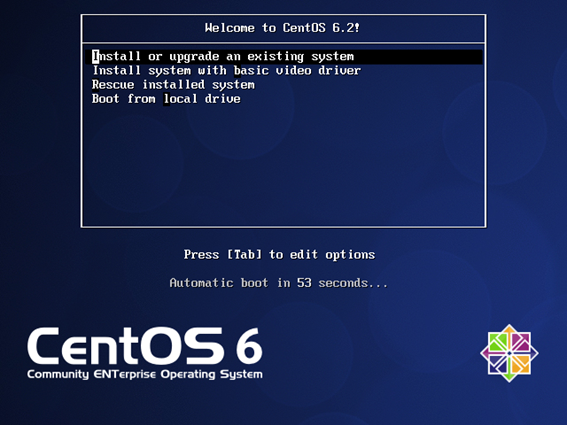
\includegraphics[width=12cm]{./Imagenes/15}
		\end{center}
	
	\end{itemize} 

\begin{itemize}
\item PASO 16:
\\Seleccionar Skip para continuar con la instalación.
		\begin{center}
		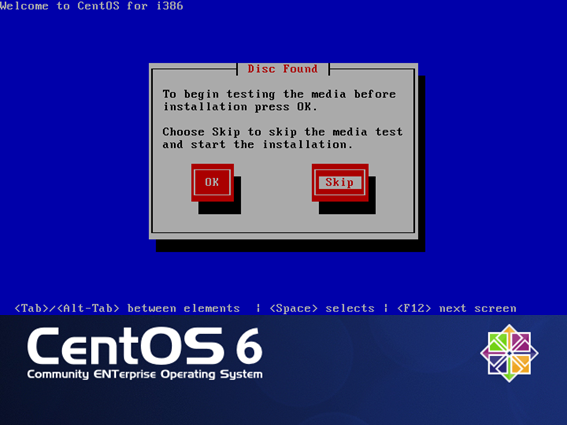
\includegraphics[width=13cm]{./Imagenes/16}
		\end{center}
	
	\end{itemize} 

\begin{itemize}
\item PASO 17:
\\Clic en Next para continuar.
		\begin{center}
		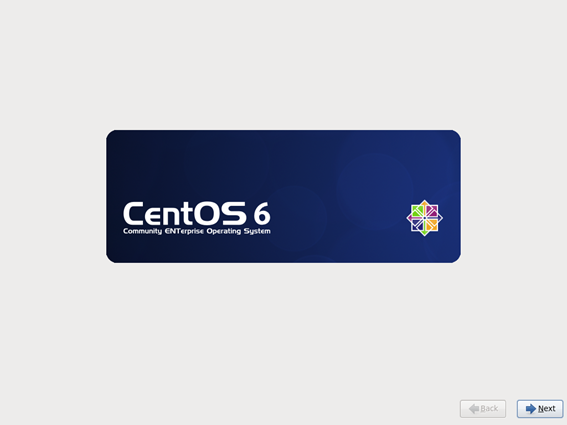
\includegraphics[width=13cm]{./Imagenes/17}
		\end{center}
	
	\end{itemize} 

\begin{itemize}
\item PASO 18:
\\Seleccionar el idioma Spanish(Español) y clic en Next.
		\begin{center}
		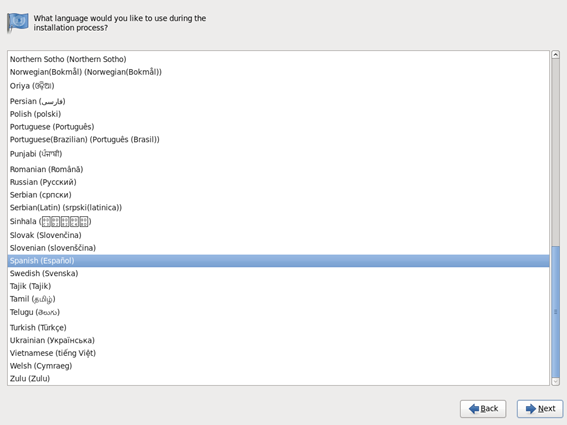
\includegraphics[width=13cm]{./Imagenes/18}
		\end{center}
	\\\
	\end{itemize} 

\begin{itemize}
\item PASO 19:
\\Seleccionar idioma del teclado en Español y clic en Siguiente.
		\begin{center}
		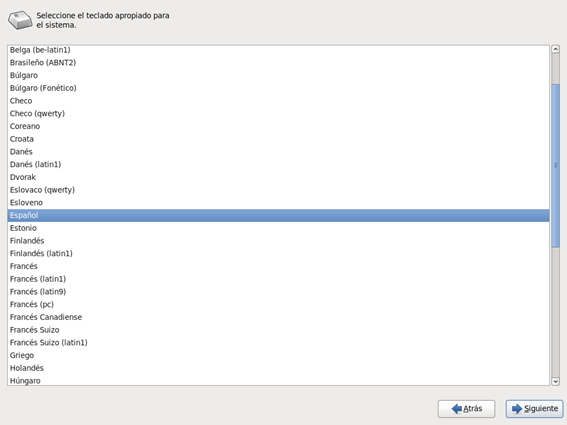
\includegraphics[width=13cm]{./Imagenes/19}
		\end{center}
	
	\end{itemize} 

\begin{itemize}
\item PASO 20:
\\Seleccionar la primera opción  Basic Storage Devices y clic en Siguiente.
		\begin{center}
		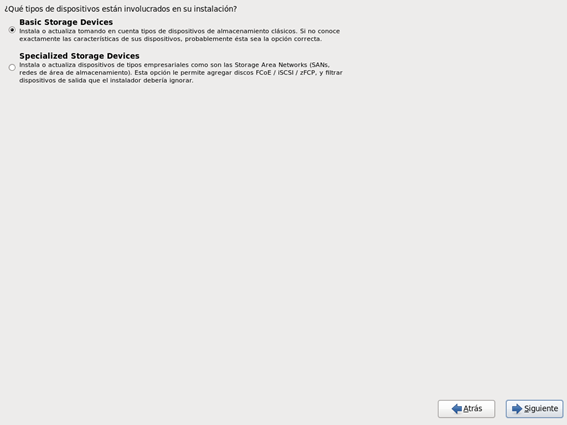
\includegraphics[width=13cm]{./Imagenes/20}
		\end{center}
	\\\
	\end{itemize} 

\begin{itemize}
\item PASO 21:
\\Seleccionar  cualquiera de las dos opciones depende del usuario.
		\begin{center}
		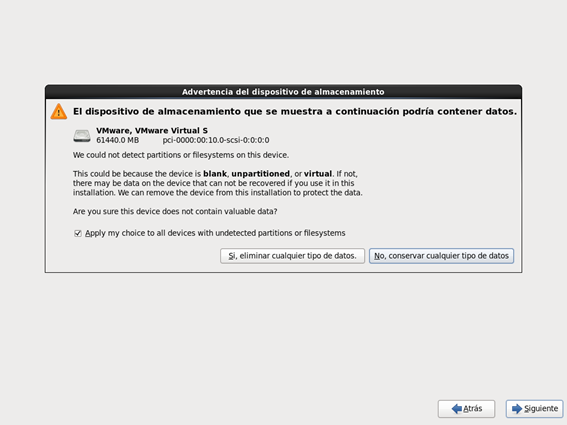
\includegraphics[width=13cm]{./Imagenes/21}
		\end{center}
	
	\end{itemize} 

\begin{itemize}
\item PASO 22:
\\Escribir un nombre del equipo o dejarlo por defecto con el nombre q sale.
		\begin{center}
		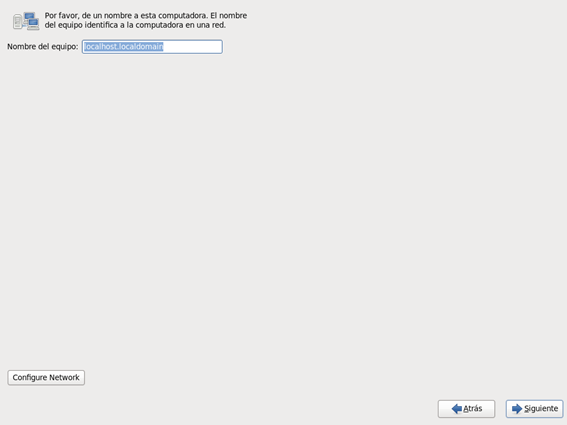
\includegraphics[width=13cm]{./Imagenes/22}
		\end{center}
	\\\
	\end{itemize} 

\begin{itemize}
\item PASO 23:
\\Seleccionar la ubicación del país en este caso America/Lima y clic en Siguiente.
		\begin{center}
		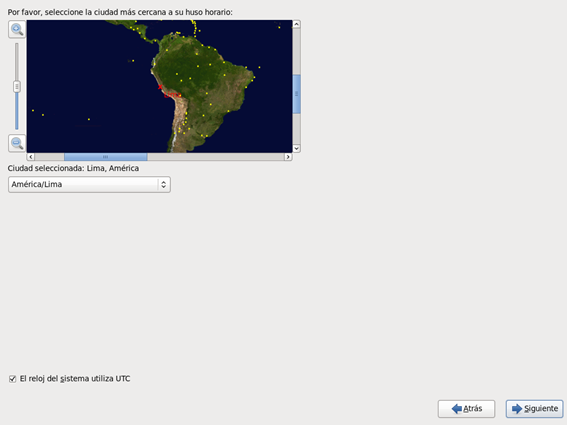
\includegraphics[width=13cm]{./Imagenes/23}
		\end{center}
	
	\end{itemize} 

\begin{itemize}
\item PASO 24:
\\Ingresar una nueva contraseña para el usuario root que viene ya creado por el CentOS.
		\begin{center}
		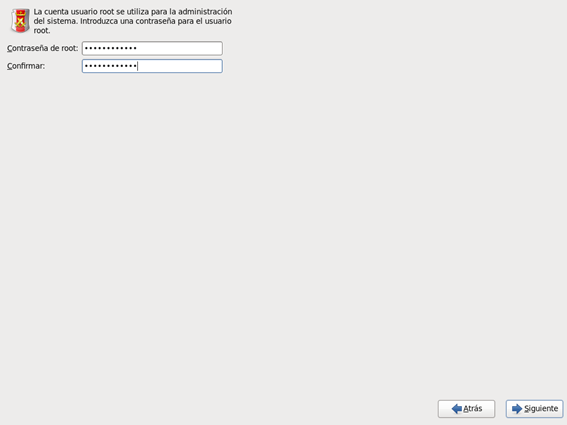
\includegraphics[width=13cm]{./Imagenes/24}
		\end{center}
	\\\
	\end{itemize} 

\begin{itemize}
\item PASO 25:
\\En este caso seleccionamos la última opción para definir manualmente nuestro diseño.
		\begin{center}
		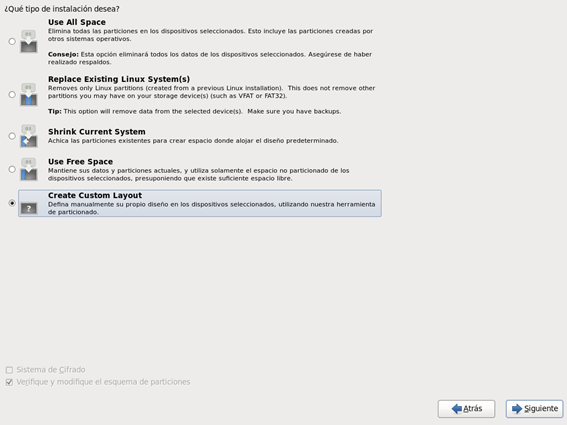
\includegraphics[width=13cm]{./Imagenes/25}
		\end{center}
	
	\end{itemize} 

\begin{itemize}
\item PASO 26:
\\Aparecerá  en blanco sin particiones nuestro dispositivo de disco duro.
		\begin{center}
		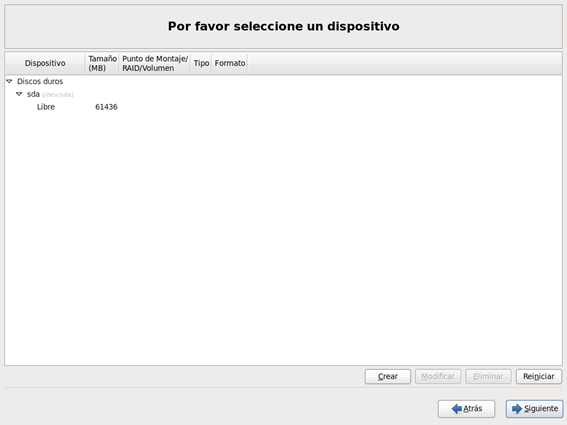
\includegraphics[width=13cm]{./Imagenes/26}
		\end{center}
	\\\
	\end{itemize} 

\begin{itemize}
\item PASO 27:
\\Clic en crear  nos saldrá una ventana y debemos crear una partición estándar.
		\begin{center}
		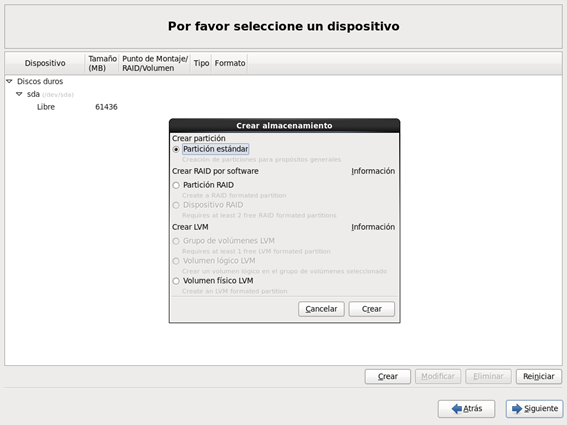
\includegraphics[width=13cm]{./Imagenes/27}
		\end{center}
	
	\end{itemize} 

\begin{itemize}
\item PASO 28:
\\Creamos primera partición  con tipo de sistema de archivos swap con 6 GB.
		\begin{center}
		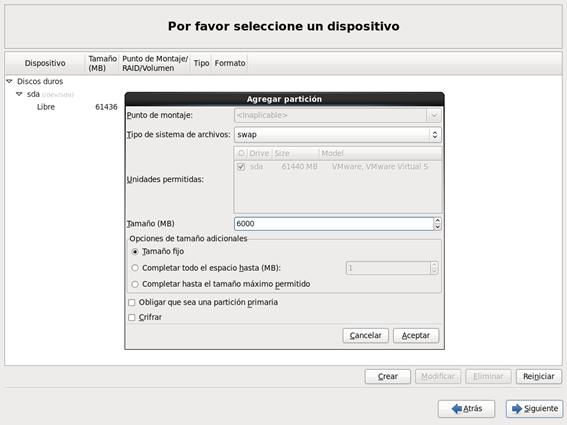
\includegraphics[width=13cm]{./Imagenes/28}
		\end{center}
	\\\
	\end{itemize} 

\begin{itemize}
\item PASO 29:
\\Creamos la segunda partición con las siguientes características /home, ext3, 20GB.
		\begin{center}
		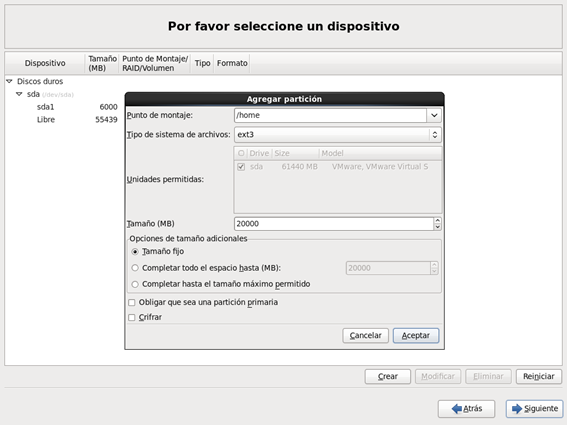
\includegraphics[width=13cm]{./Imagenes/29}
		\end{center}
	
	\end{itemize} 

\begin{itemize}
\item PASO 30:
\\Creamos la tercera partición con las siguientes características /, ext3, y todo los GB.
		\begin{center}
		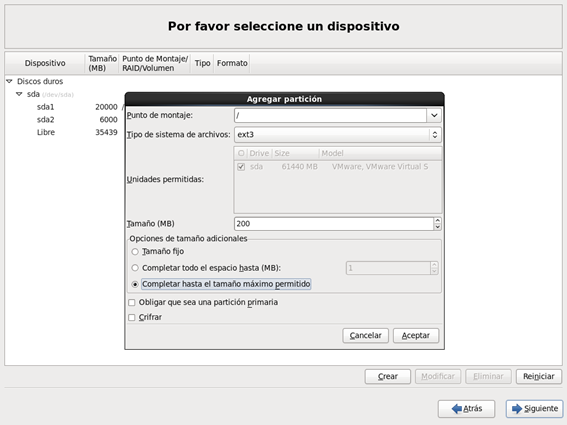
\includegraphics[width=13cm]{./Imagenes/30}
		\end{center}
	\\\
	\end{itemize} 

\begin{itemize}
\item PASO 31:
\\Una vez creado las particiones damos clic en formatear.
		\begin{center}
		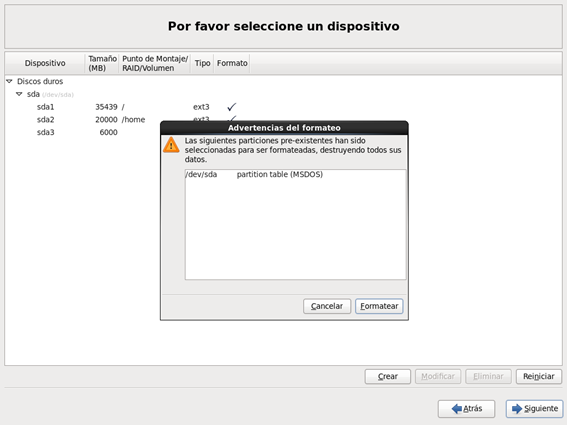
\includegraphics[width=13cm]{./Imagenes/31}
		\end{center}
	
	\end{itemize} 

\begin{itemize}
\item PASO 32:
\\Seleccionamos  la primera opción para  tener un Desktop CentOS 6.2.
		\begin{center}
		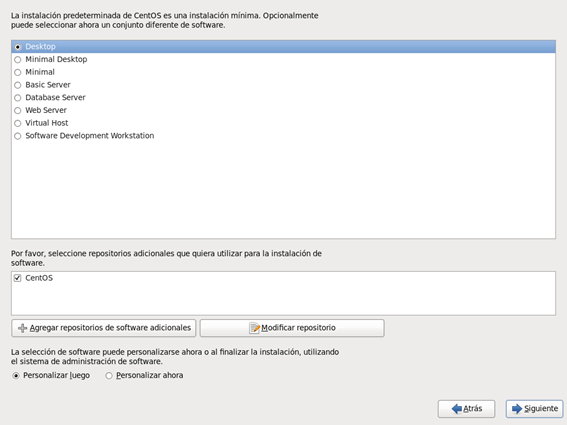
\includegraphics[width=13cm]{./Imagenes/32}
		\end{center}
	\\\
	\end{itemize} 

\begin{itemize}
\item PASO 33:
\\El proceso de la instalación tardara unos minutos.
		\begin{center}
		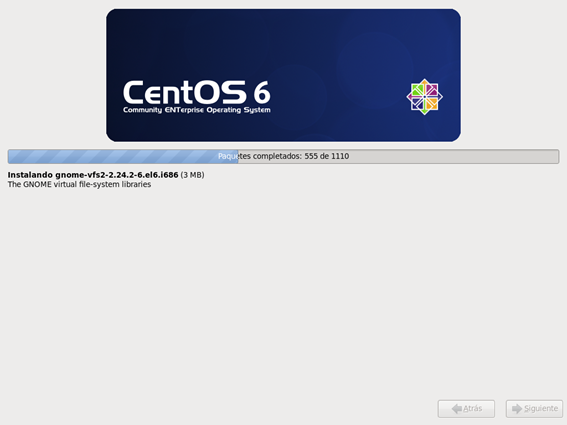
\includegraphics[width=13cm]{./Imagenes/33}
		\end{center}
	
	\end{itemize} 

\begin{itemize}
\item PASO 34:
\\Una vez finalizado la instalación finalizamos haciendo clic en reiniciar.
		\begin{center}
		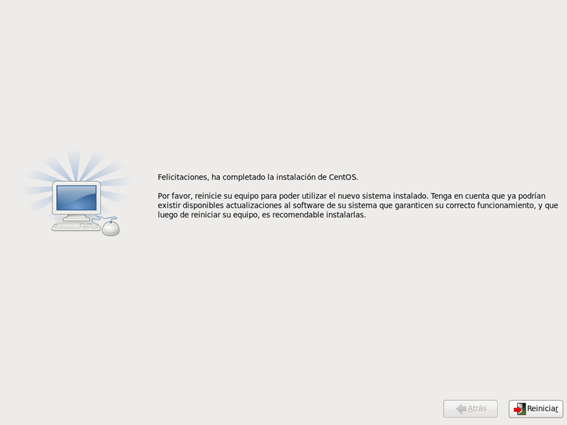
\includegraphics[width=13cm]{./Imagenes/34}
		\end{center}
	\\\
	\end{itemize} 

\begin{itemize}
\item PASO 35:
\\Tendremos una pantalla de bienvenida  y hacemos clic en Al frente..
		\begin{center}
		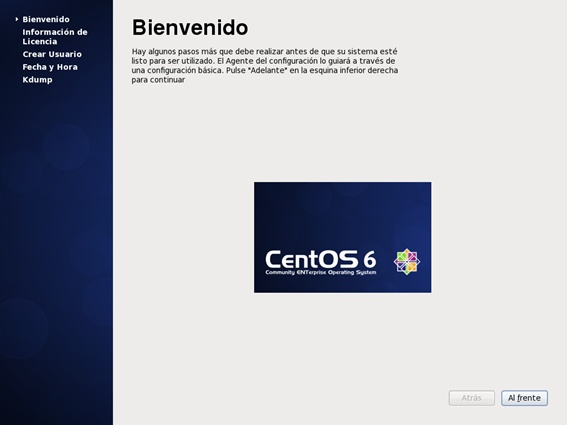
\includegraphics[width=13cm]{./Imagenes/35}
		\end{center}
	
	\end{itemize} 

\begin{itemize}
\item PASO 36:
\\Seguidamente aceptamos los acuerdos de licencia  y clic en Al Frente.
		\begin{center}
		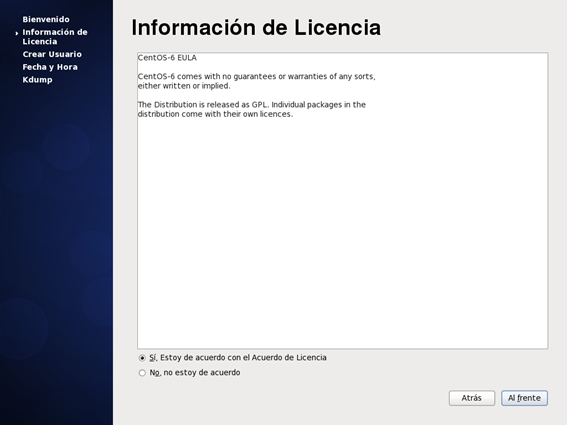
\includegraphics[width=13cm]{./Imagenes/36}
		\end{center}
	\\\
	\end{itemize} 

\begin{itemize}
\item PASO 37:
\\Creamos un usuario con su contraseña y clic en Al Frente.
		\begin{center}
		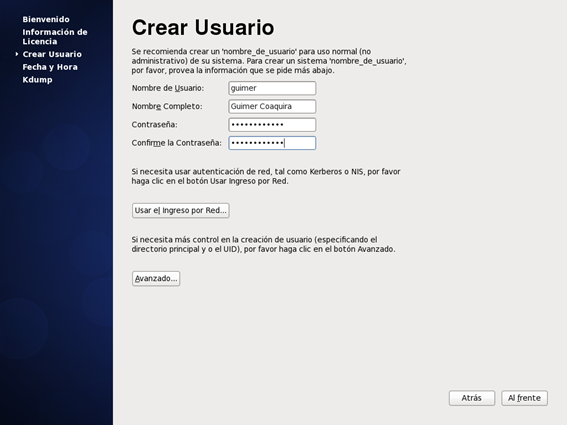
\includegraphics[width=13cm]{./Imagenes/37}
		\end{center}
	
	\end{itemize} 

\begin{itemize}
\item PASO 38:
\\Configuramos la fecha y hora del sistema y clic en Al Frente.
		\begin{center}
		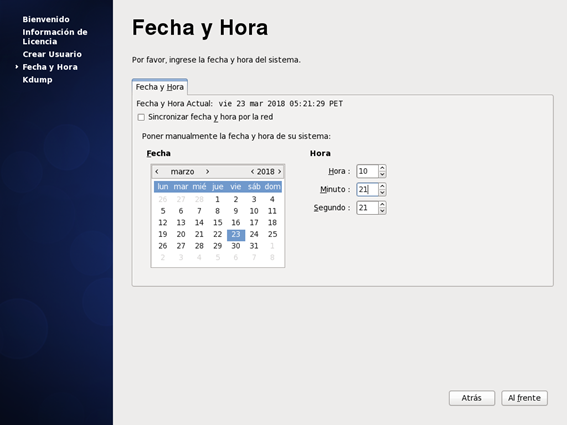
\includegraphics[width=13cm]{./Imagenes/38}
		\end{center}
		\\\
	\end{itemize} 

\begin{itemize}
\item PASO 39:
\\Clic en finalizar sin realzar ningún cambio.
		\begin{center}
		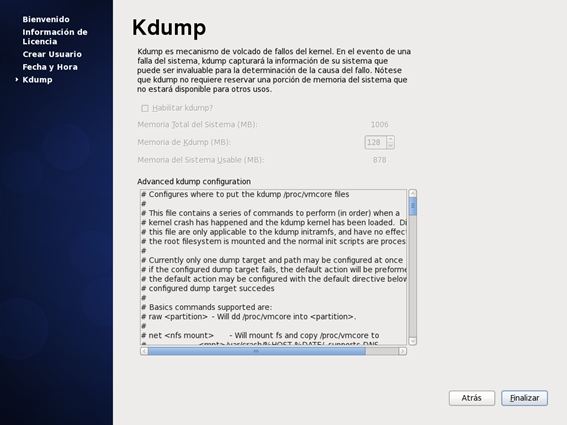
\includegraphics[width=13cm]{./Imagenes/39}
		\end{center}
	
	\end{itemize} 

\begin{itemize}
\item PASO 40:
\\Una vez iniciado nuestro sistema operativo CentOS 6.2 iniciamos sesión.
		\begin{center}
		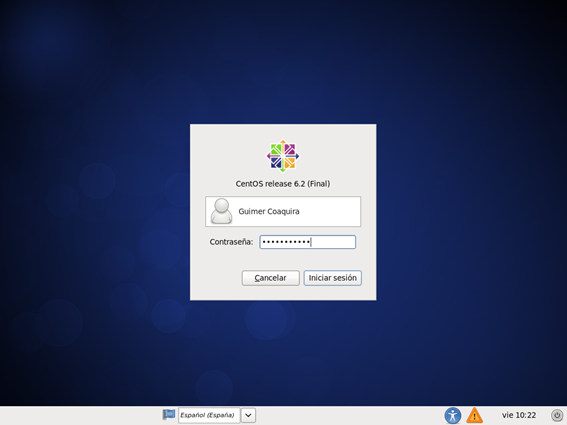
\includegraphics[width=13cm]{./Imagenes/40}
		\end{center}
		\\\
	\end{itemize} 

\begin{itemize}
\item PASO 41:
\\Finalmente ya tenemos nuestro escritorio en CentOS 6.2 con un entorno gráfico.
		\begin{center}
		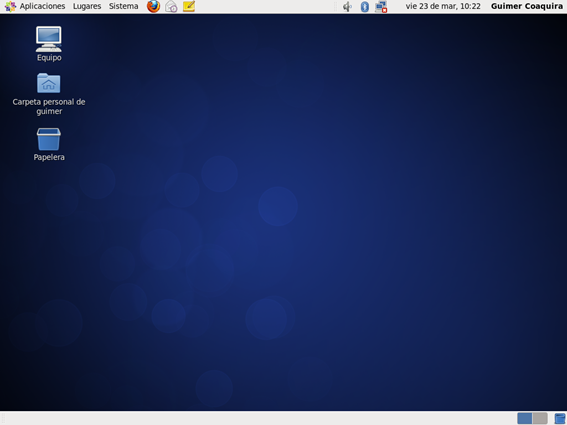
\includegraphics[width=13cm]{./Imagenes/41}
		\end{center}
	
	\end{itemize} 

